\documentclass{anstrans}

%% INCLUDING THE PREAMBLE
\usepackage[usenames,dvipsnames]{xcolor}
\usepackage{listings,amsmath}
\usepackage{microtype,todonotes}

%% CPATION SETUP
\usepackage{caption}
\usepackage{subcaption}
\captionsetup{belowskip=12pt,aboveskip=4pt}

\usepackage{fancyvrb}
\VerbatimFootnotes

%% HYPERLINKS
\usepackage[debug]{hyperref}

%% GRAPHICS RELATED
\usepackage{graphicx}
\usepackage[outdir=./tmp/]{epstopdf}
\graphicspath{{../images/}{./}{./tmp/}}
\DeclareGraphicsExtensions{.eps, .pdf, .jpeg, .png}

%% USER COMMANDS
\newcommand{\iso}[2]{${}^{#2}${#1}}
\newcommand{\figurewidth}{0.45\textwidth}
\newcommand{\micron}{$\mu$m}

%%%%%%%%%%%%%%%%%%%%%%%%%%%%%%%%%%%%%%%%%%%%%%%%%%%%%%%%%%%%%%%%%%%%%%%%%%%
%                                                                         %
%                        AUTHOR, TITLE, and ABSTRACT                      %
%                                                                         %
%%%%%%%%%%%%%%%%%%%%%%%%%%%%%%%%%%%%%%%%%%%%%%%%%%%%%%%%%%%%%%%%%%%%%%%%%%%
\title{An Improved ANS Transaction Template}
\author{Matthew J. Urffer \and L. F. Miller}
\institute{
Department of Nuclear Engineering, University of Tennessee, Knoxville, TN, 37916
}
\email{murffer@utk.edu \and lfmiller@utk.edu}


\begin{document}
%%%%%%%%%%%%%%%%%%%%%%%%%%%%%%%%%%%%%%%%%%%%%%%%%%%%%%%%%%%%%%%%%%%%%%%%%%%
%                                                                         %
%                               INTRODUCTION                              %
%                                                                         %
%%%%%%%%%%%%%%%%%%%%%%%%%%%%%%%%%%%%%%%%%%%%%%%%%%%%%%%%%%%%%%%%%%%%%%%%%%%
\section{Introduction}
The Department of Homeland Security (DHS) continues to fund research (through the Domestic Nuclear Detection Office (DNDO)) for replacement detectors for nuclear material.
These detectors are designed to replace the \iso{He}{3} detectors currently installed as radation portal monitors.
DHS / DNDO (along with PNNL) has determined a set of objectives that replacement technologies should meet (summerized in Table ~\ref{tab:DHSCriteria}).
\begin{table}[h]
    \caption{Replacement Detector Requirements  }
    %\caption{Replacement Detector Requirements \protect\cite{kouzes_neutron_1999} }
	\centering
	\begin{tabular}{p{0.2\textwidth} | p{0.2\textwidth} }
	Parameter & Specification \\
	\hline
	\hline
	Absolute neutron detection efficiency & 2.5 cps/ng of ${}^{252}$Cf \\
	Intrinsic gamma-neutron detection efficiency & $ \epsilon_{int,\gamma n}\leq 10^{-6}$ \\
	Gamma absolute rejection ratio for neutrons (GARRn) & $ 0.9 \leq \text{ GARRn }\leq$ 1.1 at 10 mR/h exposure \\
	Cost &  \$ 30,000 per system \\
	\hline
	\end{tabular}
    \label{tab:DHSCriteria}
\end{table}
These detectors must be able to effectively discriminate between gammas (which can occur in medical isotopes) and neutrons (indictive of special nuclear material).

A possible replacment technology being investigated is \iso{Li}{6} embeded in a scinilating polymer matrix.

The effective discrimination between neutrons and gammas is necessary for replacement detectors 
%%%%%%%%%%%%%%%%%%%%%%%%%%%%%%%%%%%%%%%%%%%%%%%%%%%%%%%%%%%%%%%%%%%%%%%%%%%
%                                                                         %
%                                 THEORY                                  %
%                                                                         %
%%%%%%%%%%%%%%%%%%%%%%%%%%%%%%%%%%%%%%%%%%%%%%%%%%%%%%%%%%%%%%%%%%%%%%%%%%%
\section{Theory}
Neutron detectors often utilize a material doped with an isotope of large thermal cross section for absorption such as \iso{Li}{6} or \iso{B}{10}. 
When these materials absorb a neutron the nucleus of the isotope becomes unstable and fissions into reaction products.
These reaction products (having an initial kinetic energy equal to the Q-value of the neutron absorption reaction) travel through the material, transferring their kinetic energy to the material.
Photon interactions in the detector occur when a photon scatters off a single electron in a Compton scattering event and transfers a portion of its energy to the electron predominately through Compton scattering.
This Compton electron then produces a cascade of secondary electrons in the material, which, depending upon the energy, may or may not deposit a majority of its energy in the detector.
The difference in the transfer of kinetic energy from charged particle to electrons and from photon interactions (Compton scattering) to electrons introduces an opportunity to exploit the difference in energy deposition in order to maximize the discrimination between neutron and photon interactions in a detector.

%%%%%%%%%%%%%%%%%%%%%%%%%%%%%%%%%%%%%%%%%%%%%%%%%%%%%%%%%%%%%%%%%%%%%%%%%%%
%                                                                         %
%                       DESCRIPTION OF WORK                               %
%                                                                         %
%%%%%%%%%%%%%%%%%%%%%%%%%%%%%%%%%%%%%%%%%%%%%%%%%%%%%%%%%%%%%%%%%%%%%%%%%%%
\section{Description of Work}
The energy deposition was investigated using simulation and then benchmarking the simulation against the measured performance of the detector.
\subsection{Detector Simulation}

\subsection{Fabricated Detector Measurements}
The pulse height of a radiation event is proportional to the energy deposition of the event\cite{birks_scintillations_1951}.

Samples are mounted to a Philips XP2202B 10 stage PMT with silicone based optical grease (Saint Gobain BC-630), which is attached to a Canberra 2007P base (also serving as a preamplifier).   
The PMT’s voltage is supplied by an Ortec 556 high voltage power supply, with the power being supplied to the Canberra 2007P pre amplifier base by the Ortec 571 amplifier.  
The output signal of the Canberra 2007P base feeds into an Ortec 572A amplifier for pulse shaping and amplification. 
The amplified signal is then inputted to an Ortec 926 MCB-ADC, and can then be read using the MAESTRO-32 software. 
A schematic of the setup is shown in Figure ~\ref{fig:ElectronicsSpectra}.
\begin{figure}
	\centering
	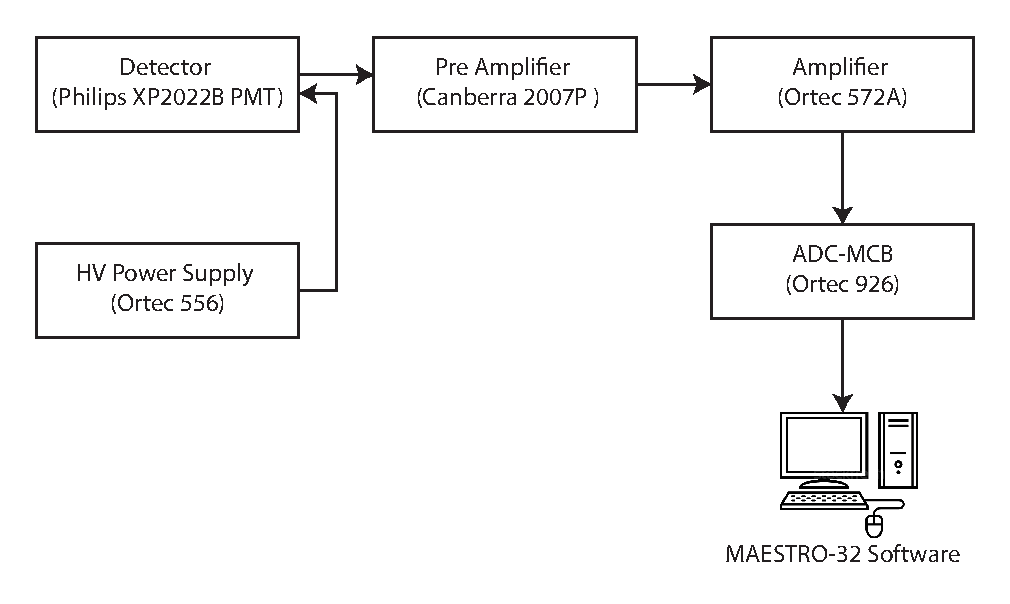
\includegraphics[width=\figurewidth]{ElectronicsSpectra}
	\caption{Pulse height measurment electronics}
	\label{fig:ElectronicsSpectra}
\end{figure}
A 100 $\mu$Ci \iso{60}{Co} source was used to measure the gamma energy deposition of the films, while a moderated \iso{252}{Cf} source was used for the neutrons.
The \iso{252}{Cf} irridiator contains two detector wells; a lead well and a cadmium well.
The lead well measures the reponse of neutron of all energies, while the cadmium well measures the responses of fast neutrons.
The two responses are then subtracted, as shwon in Figure ~\ref{fig:SimPbCdSpectra}.
	\begin{figure}
		\centering
		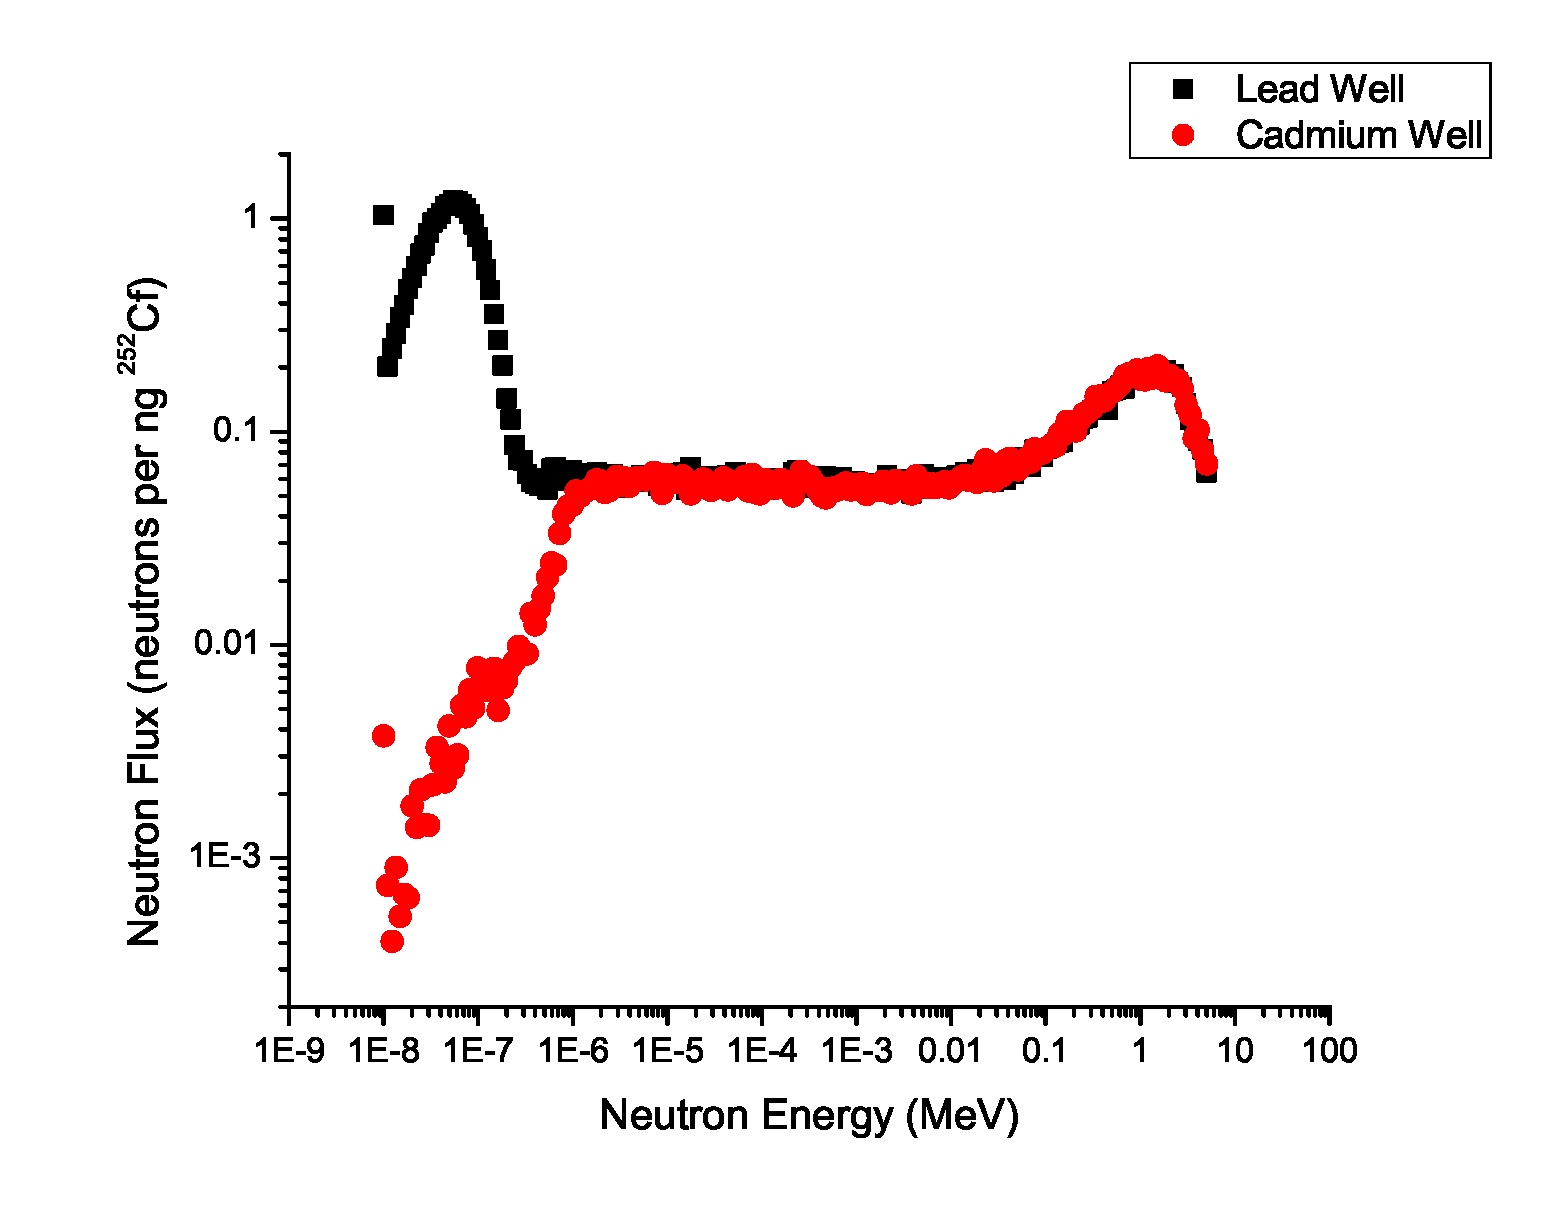
\includegraphics[width=\figurewidth]{Graph19N}
		\caption{Simulated Lead and Cadmium Well Spectra. The difference between the two spectra is the thermal neutron response and is what is measured.}
		\label{fig:SimPbCdSpectra}
	\end{figure}
%%%%%%%%%%%%%%%%%%%%%%%%%%%%%%%%%%%%%%%%%%%%%%%%%%%%%%%%%%%%%%%%%%%%%%%%%%%
%                                                                         %
%                     RESULTS and ANALYSIS                                %
%                                                                         %
%%%%%%%%%%%%%%%%%%%%%%%%%%%%%%%%%%%%%%%%%%%%%%%%%%%%%%%%%%%%%%%%%%%%%%%%%%%
\section{Results and Analysis}
%G4EDep_Co60_Fraction.eps
%G4EDep_LightYeild_Co60.eps
%G4EDep_LightYield_Co60.eps
%G4EDep_LightYield_Neutron.eps
%G4EDep_Neutrons_Fraction.eps
%G4EDep_NGComparison.eps
%G4EDep_NGComparison_SimChannel.eps
%PS_EDepSim_Co60.eps
%PS_EDepSim_Neutron.eps
\begin{figure}[h]
    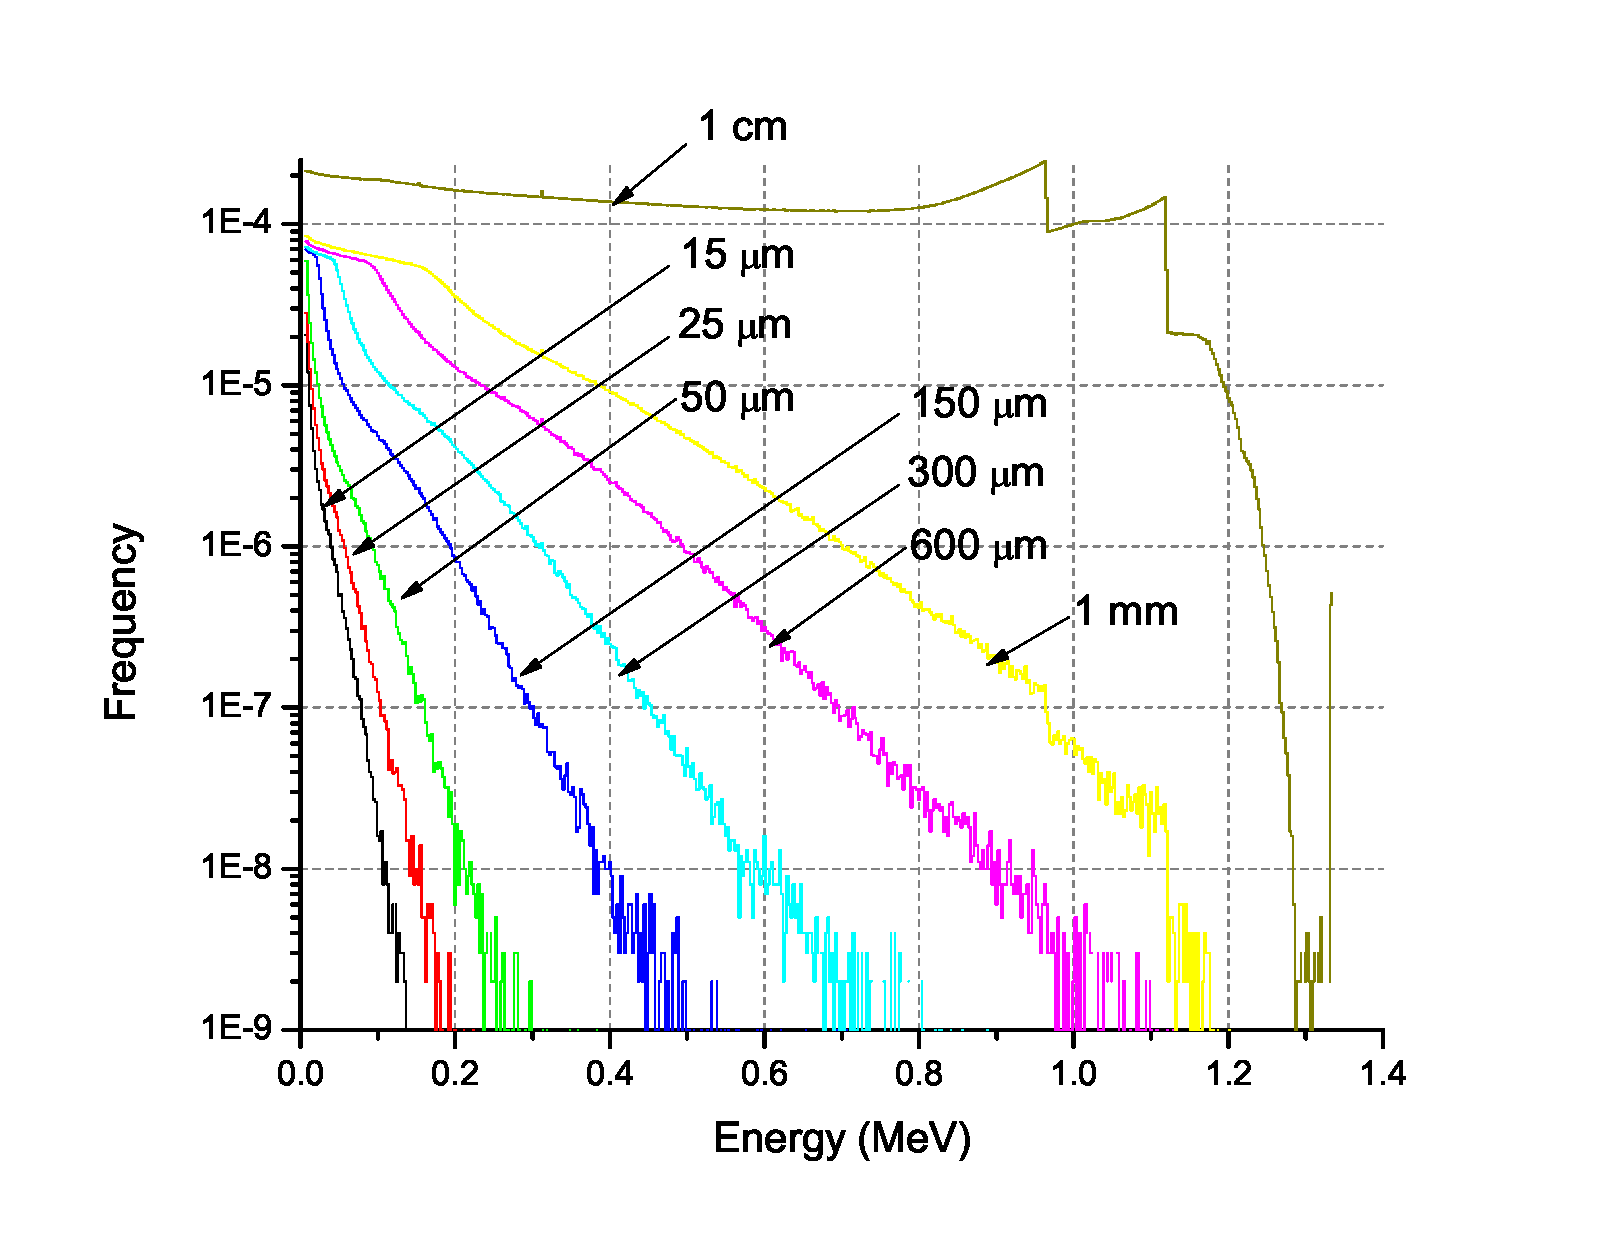
\includegraphics[width=\figurewidth]{PS_EDepSim_Co60}
	\caption{Simulated Energy Depositon for a Single Film (gammas)}
    \label{fig:SimEDepGamma}
\end{figure}
\begin{figure}[h]
    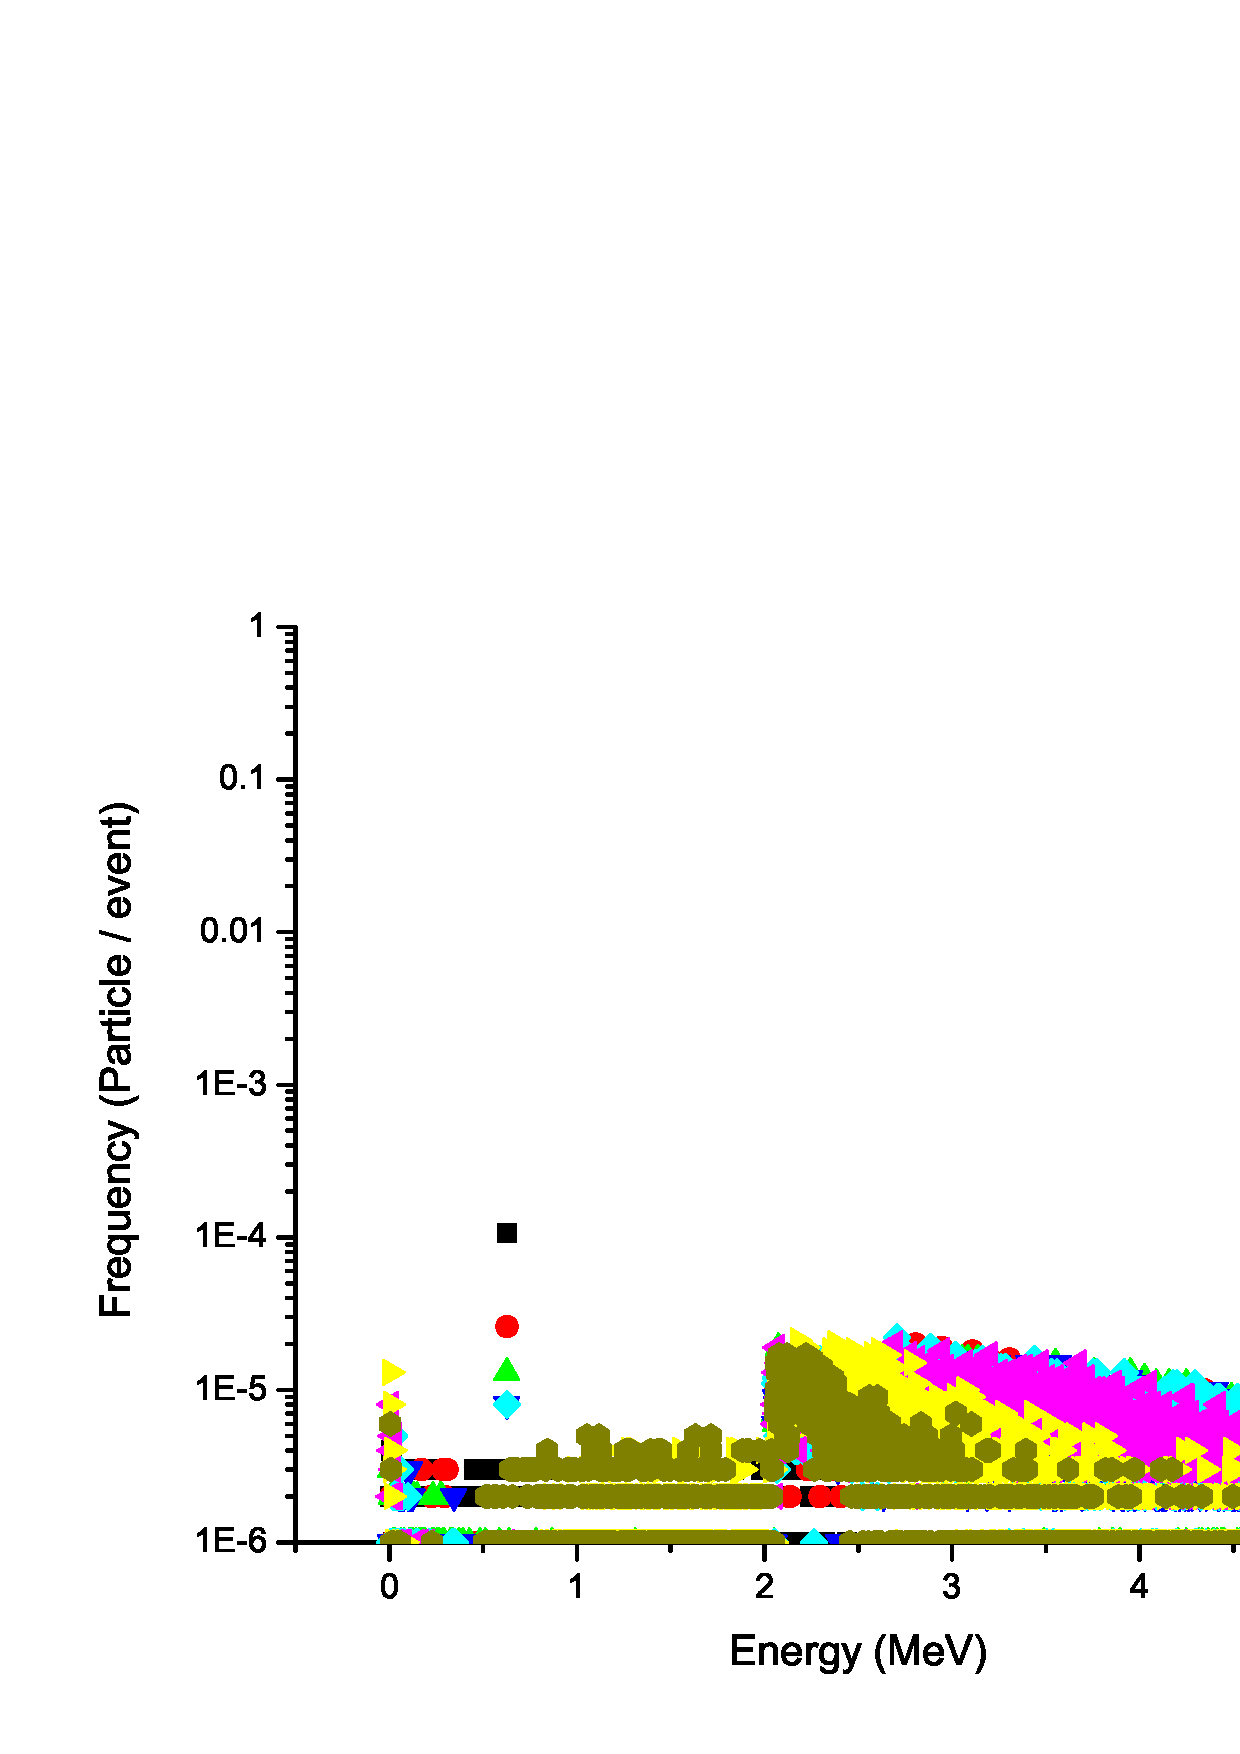
\includegraphics[width=\figurewidth]{PS_EDepSim_Neutron}
	\caption{Simulated Energy Depositon for a Single Film (neutron)}
    \label{fig:SimEDepGamma}
\end{figure}
The results were interesting, so interesting in fact that we have decided to
present them here.

%%%%%%%%%%%%%%%%%%%%%%%%%%%%%%%%%%%%%%%%%%%%%%%%%%%%%%%%%%%%%%%%%%%%%%%%%%%
%                                                                         %
%                             CONCLUSIONS                                 %
%                                                                         %
%%%%%%%%%%%%%%%%%%%%%%%%%%%%%%%%%%%%%%%%%%%%%%%%%%%%%%%%%%%%%%%%%%%%%%%%%%%
\section{Conclusions}

The included ANS style file and this clear example file are a panacea for
the hours of headache that invariably results from formatting a document in
Microsoft Word.


%%%%%%%%%%%%%%%%%%%%%%%%%%%%%%%%%%%%%%%%%%%%%%%%%%%%%%%%%%%%%%%%%%%%%%%%%%%%%%%%
\section{Acknowledgments}
This works was supported by the Domestic Nuclear Detection Office (DNDO) through award 003387891.
Any opinions, fidinings, and conclusions or rrecommendations expressed in this material are those of the authors and do necessarily reflect the views of DNDO.

%%%%%%%%%%%%%%%%%%%%%%%%%%%%%%%%%%%%%%%%%%%%%%%%%%%%%%%%%%%%%%%%%%%%%%%%%%%%%%%%
\bibliographystyle{ans}
\bibliography{bibliography}
\end{document}

